% Four slides: cycle rank, the merged-sea networks, GCC and GLCC, and cyclones.
% To use in the main deck: copy the four frames below, the figures/ folder,
% and the packages and \tikzset block marked "needed by the frames" into the main preamble.
\documentclass[aspectratio=169]{beamer}

% needed by the frames
\usepackage{amsmath}
\usepackage{tikz}
\usetikzlibrary{arrows.meta}
\graphicspath{{figures/}}
\tikzset{
  cr-node/.style={circle, draw=blue!50!black, fill=blue!10, inner sep=1.5pt, minimum size=15pt, font=\scriptsize},
  cr-link/.style={line width=1.1pt, blue!45!black},
  cr-new/.style={line width=1.3pt, red!75!black},
}

\setbeamertemplate{navigation symbols}{}

\begin{document}

% ---------------------------------------------------------------- slide 1
\begin{frame}{Cycle rank: counting loops}
\begin{columns}[c,onlytextwidth]
\begin{column}{0.42\textwidth}
\textbf{Cycle rank} is the number of independent loops in a channel network:
\[ \mu = E - N + C \]
{\small $E$ links, $N$ nodes, $C$ connected components.}

\vspace{4mm}
\begin{itemize}\setlength{\itemsep}{3pt}
  \item $\mu = 0$: a branching tree, like a river.
  \item Every extra link closes one more loop.
\end{itemize}
\end{column}

\begin{column}{0.56\textwidth}
\centering
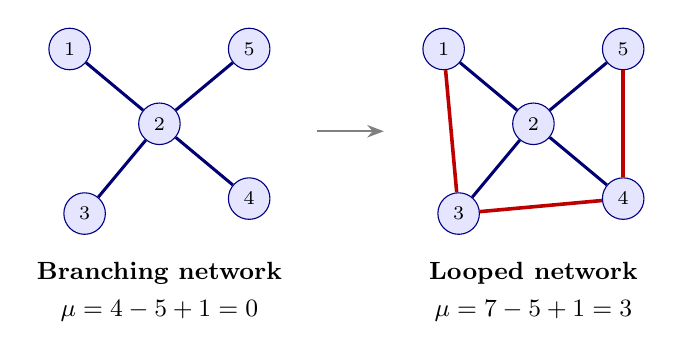
\begin{tikzpicture}[scale=0.95]
  % branching network
  \begin{scope}
    \node[cr-node] (1) at (0,2.6) {1}; \node[cr-node] (2) at (1.2,1.6) {2}; \node[cr-node] (3) at (0.2,0.4) {3};
    \node[cr-node] (4) at (2.4,0.6) {4}; \node[cr-node] (5) at (2.4,2.6) {5};
    \draw[cr-link] (1) -- (2); \draw[cr-link] (2) -- (3); \draw[cr-link] (2) -- (4); \draw[cr-link] (2) -- (5);
    \node[font=\small\bfseries] at (1.2,-0.4) {Branching network};
    \node[font=\small] at (1.2,-0.9) {$\mu = 4 - 5 + 1 = 0$};
  \end{scope}
  \draw[-{Stealth[length=6pt]}, thick, gray] (3.3,1.5) -- (4.2,1.5);
  % looped network: the same nodes, three more links
  \begin{scope}[xshift=5.0cm]
    \node[cr-node] (1) at (0,2.6) {1}; \node[cr-node] (2) at (1.2,1.6) {2}; \node[cr-node] (3) at (0.2,0.4) {3};
    \node[cr-node] (4) at (2.4,0.6) {4}; \node[cr-node] (5) at (2.4,2.6) {5};
    \draw[cr-link] (1) -- (2); \draw[cr-link] (2) -- (3); \draw[cr-link] (2) -- (4); \draw[cr-link] (2) -- (5);
    \draw[cr-new] (1) -- (3); \draw[cr-new] (3) -- (4); \draw[cr-new] (4) -- (5);
    \node[font=\small\bfseries] at (1.2,-0.4) {Looped network};
    \node[font=\small] at (1.2,-0.9) {$\mu = 7 - 5 + 1 = 3$};
  \end{scope}
\end{tikzpicture}

\vspace{1mm}
{\scriptsize Red: the three extra links, each closing one loop.\par}
\end{column}
\end{columns}

\vspace{4mm}
\alert{\small The Sundarbans tidal network is loop-rich and interconnected, unlike the tree-like structure of conventional rivers.}
\end{frame}

% ---------------------------------------------------------------- slide 2
\begin{frame}{All outlets merged into one sea node}
\centering
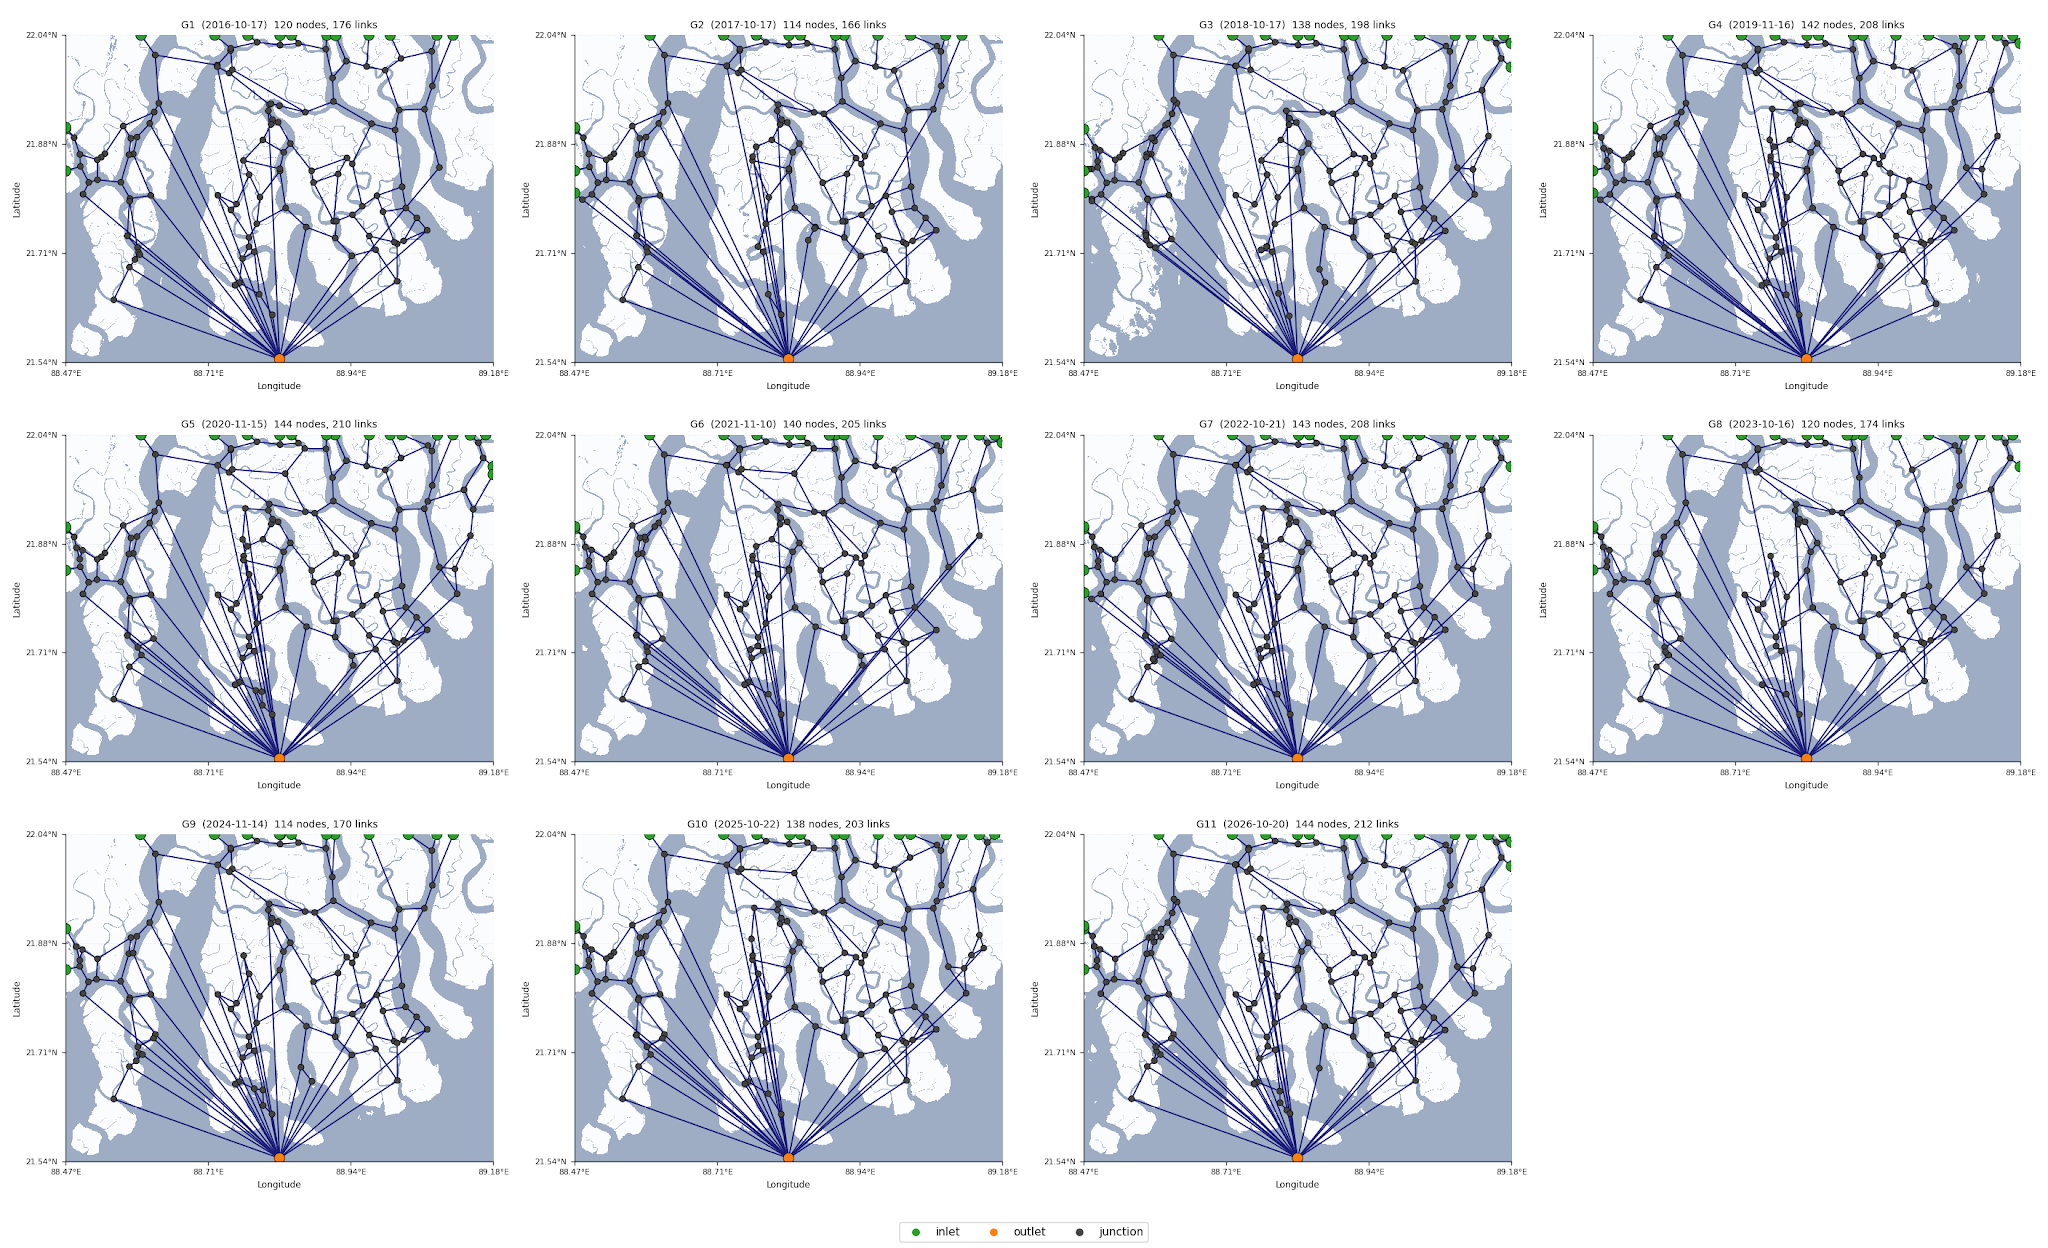
\includegraphics[width=0.84\textwidth]{networks_merged_sea.png}

\vspace{1mm}
\small Every outlet is joined to a single sea node (orange). The 11 networks have 114--144 nodes and 166--212 links.
\end{frame}

% ---------------------------------------------------------------- slide 3
\begin{frame}{Is the channel network connected?}
\centering
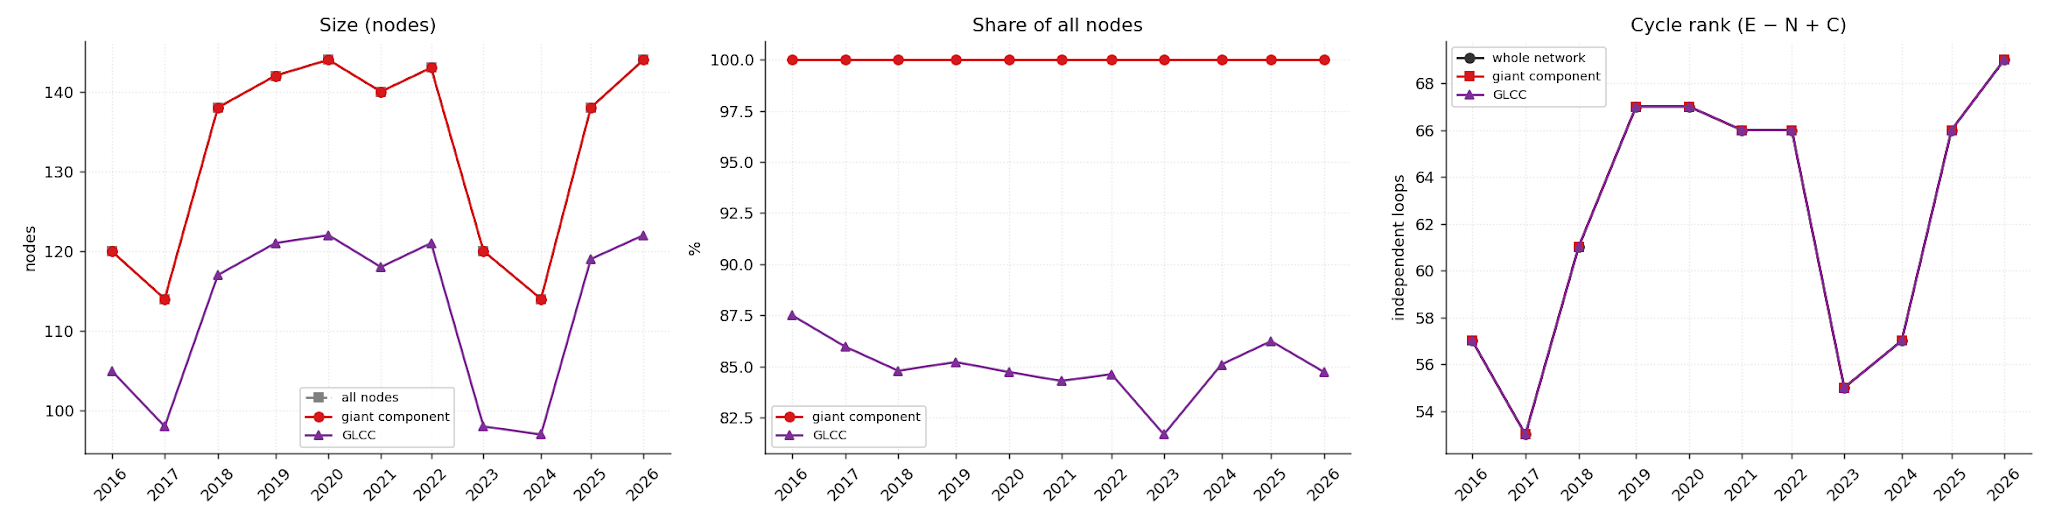
\includegraphics[width=\textwidth]{gcc_glcc_top.png}

\vspace{1mm}
\begin{columns}[T,onlytextwidth]
\begin{column}{0.48\textwidth}
\small
\textbf{Giant connected component (GCC):} the largest piece in which every node can reach every other.

\vspace{1mm}
\alert{It holds all nodes in every year.}
\end{column}
\begin{column}{0.48\textwidth}
\small
\textbf{Giant loop-connected core (GLCC):} the GCC with dead-end nodes (one link) removed. It is the backbone where water has alternative routes.

\vspace{1mm}
\alert{82--88\% of nodes, carrying every loop.}
\end{column}
\end{columns}
\end{frame}

% ---------------------------------------------------------------- slide 4
\begin{frame}{Cyclones and network connectivity}
\begin{columns}[c,onlytextwidth]
\begin{column}{0.52\textwidth}
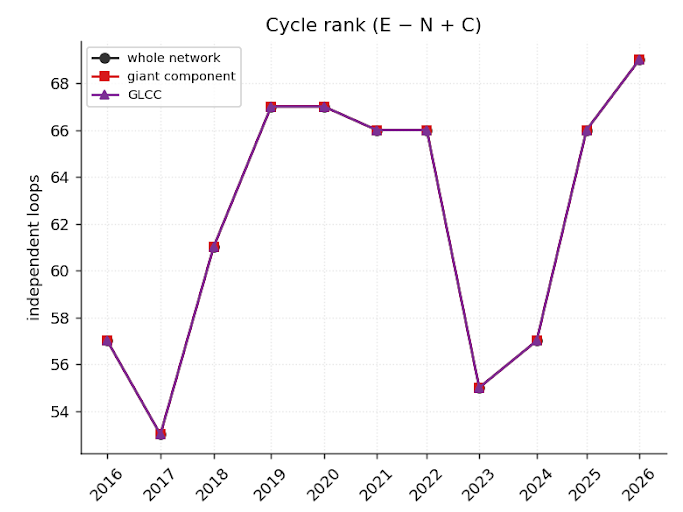
\includegraphics[width=\linewidth]{cycle_rank_merged.png}
\end{column}
\begin{column}{0.46\textwidth}
\centering
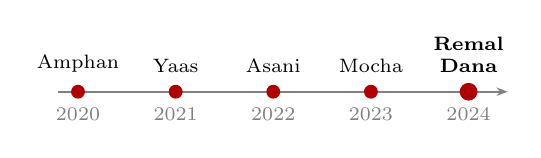
\begin{tikzpicture}[x=0.62cm, y=1cm, every node/.style={font=\scriptsize}]
  \draw[-{Stealth[length=4pt]}, thick, gray] (-0.4,0) -- (8.8,0);
  \foreach \yr/\lab in {0/2020, 2/2021, 4/2022, 6/2023, 8/2024}
    { \draw[gray] (\yr,0.08) -- (\yr,-0.08); \node[below, gray] at (\yr,-0.08) {\lab}; }
  \fill[red!70!black] (0,0) circle (2.5pt);   \node[above, align=center] at (0,0.12) {Amphan};
  \fill[red!70!black] (2,0) circle (2.5pt);   \node[above, align=center] at (2,0.12) {Yaas};
  \fill[red!70!black] (4,0) circle (2.5pt);   \node[above, align=center] at (4,0.12) {Asani};
  \fill[red!70!black] (6,0) circle (2.5pt);   \node[above, align=center] at (6,0.12) {Mocha};
  \fill[red!70!black] (8,0) circle (3.2pt);   \node[above, align=center] at (8,0.12) {\textbf{Remal}\\\textbf{Dana}};
\end{tikzpicture}

\vspace{1mm}
{\scriptsize Recent Bay of Bengal cyclones\par}

\vspace{4mm}
\raggedright\small
\begin{itemize}\setlength{\itemsep}{3pt}
  \item Cycle rank rises after the 2024 cyclones (Remal, Dana): 57 in 2024, 66 in 2025, 69 in 2026.
  \item This suggests the cyclones reshaped the tidal channels and added loops.
\end{itemize}

\vspace{2mm}
{\scriptsize The 2023--24 values are sensitive to the water threshold, so treat this link as a hypothesis.\par}
\end{column}
\end{columns}
\end{frame}

\end{document}
